\begin{frame}{Levels (Orders) of Protein Structure}
	\vspace{-0.5em}
	\begin{center}
		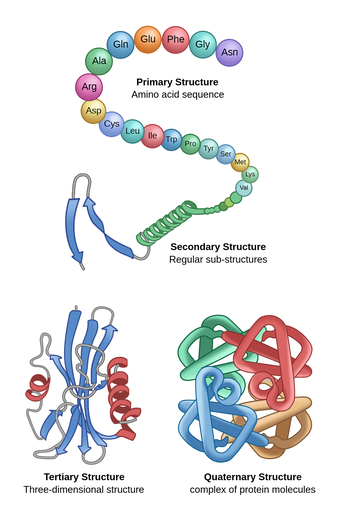
\includegraphics[trim={0 0 0 2em},clip,scale=0.46]{images/protein_structure_levels.png}
	\end{center}
	\vspace{-1.5em}
	\crediturl{Image}{https://theory.labster.com/protein-structure}
\end{frame}

\begin{frame}{Primary Protein Structure}
	\begin{center}
		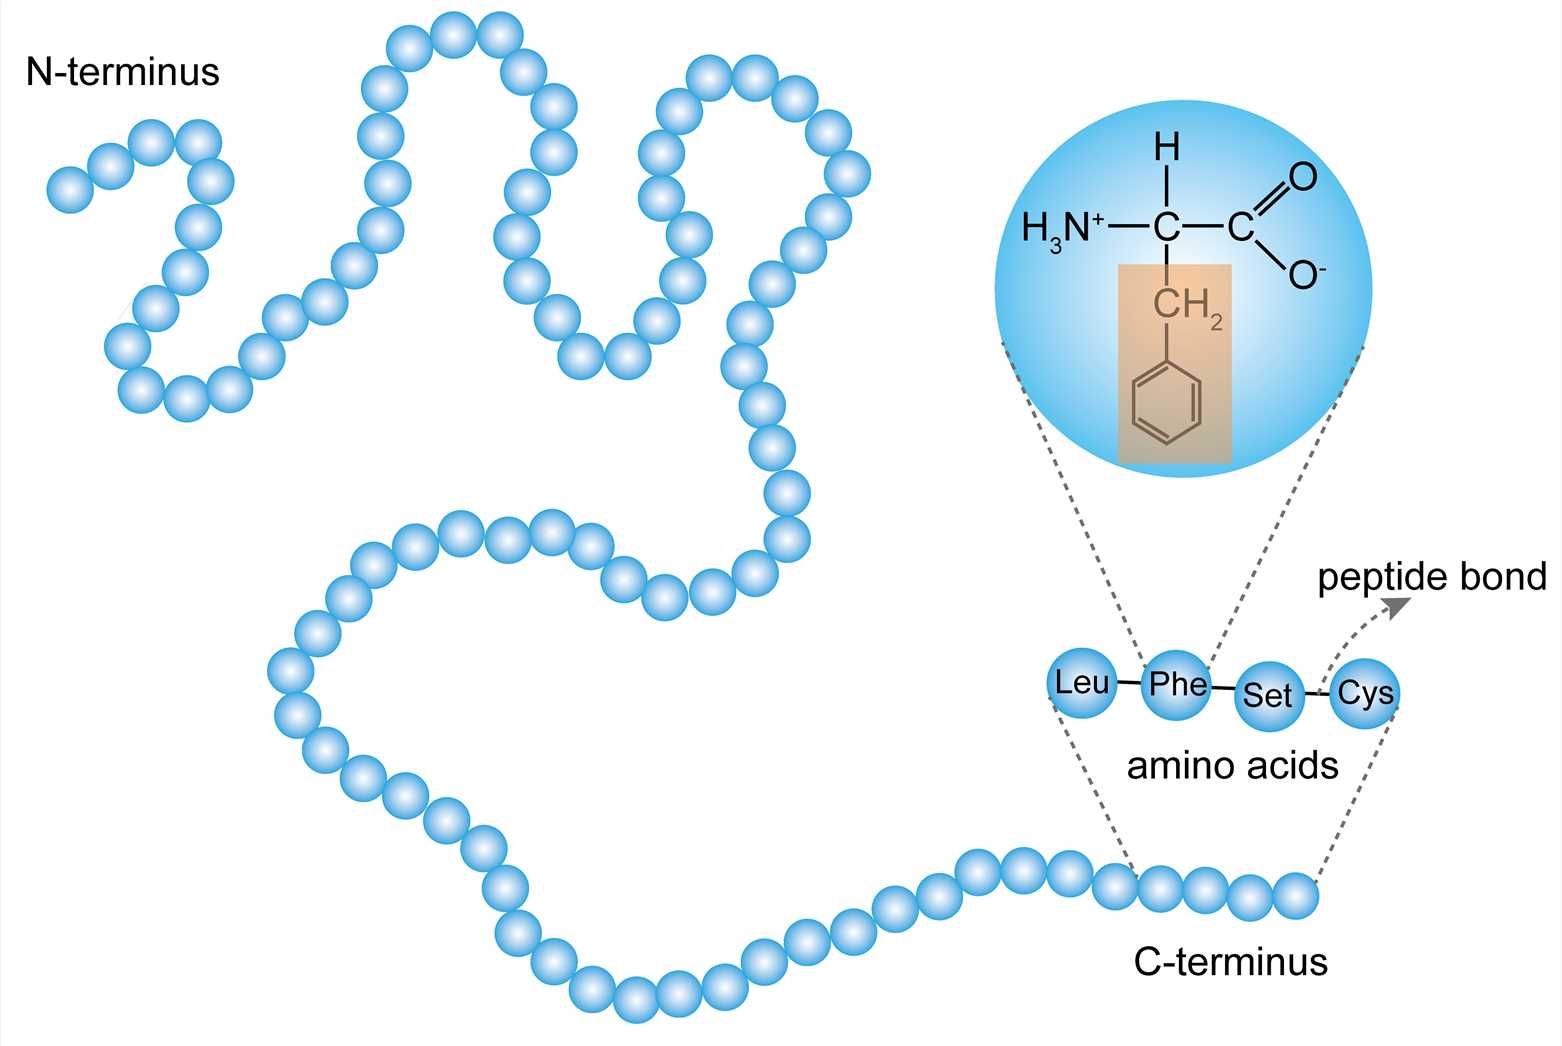
\includegraphics[scale=0.22]{images/primary_protein_structure.jpg}
	\end{center}
	\crediturl{Image}{https://www.creative-biostructure.com/levels-of-protein-structure.htm}
	\begin{itemize}
		\item One-dimensional sequence
		\item Chain of amino acids, polypeptide chain
		\item 20 possible amino acids
	\end{itemize}
\end{frame}

\begin{frame}{Secondary Protein Structure}
	\begin{center}
		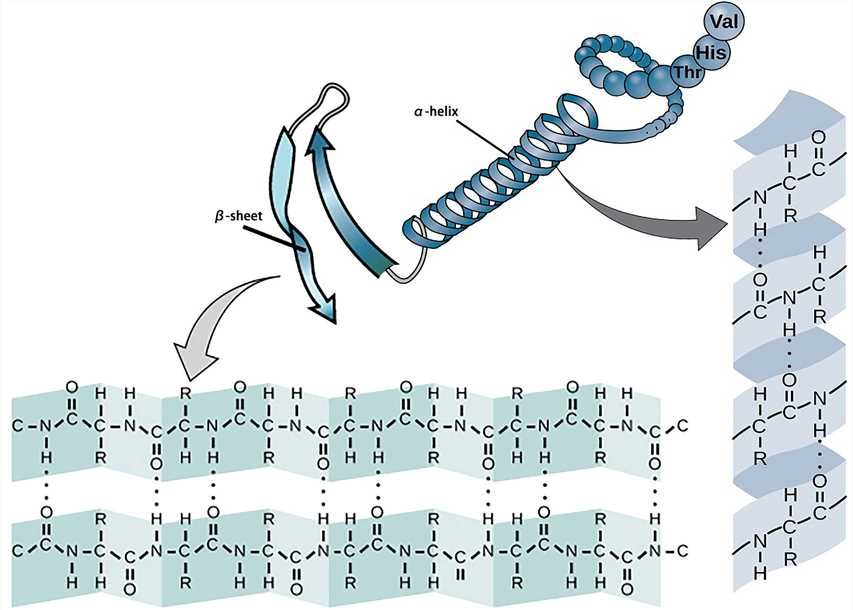
\includegraphics[scale=0.44]{images/secondary_protein_structure.jpg}
	\end{center}
	\crediturl{Image}{https://www.creative-biostructure.com/levels-of-protein-structure.htm}
	\begin{itemize}
		\item Protein sequence folds due to hydrogen bonds in the peptide backbone
	\end{itemize}
\end{frame}

\begin{frame}{Tertiary Protein Structure}
	\begin{center}
		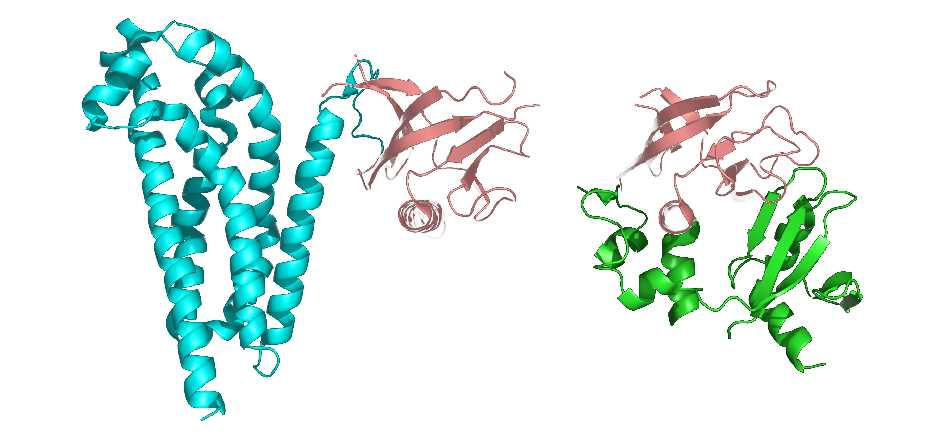
\includegraphics[scale=0.49]{images/tertiary_protein_structure.png}
	\end{center}
	\crediturl{Image}{https://www.creative-biostructure.com/levels-of-protein-structure.htm}
	\begin{itemize}
		\item Three-dimensional
		\item Protein folds and curls w.r.t. secondary structures due to side chain interactions
	\end{itemize}
\end{frame}

\begin{frame}{Quaternary Protein Structure}
\begin{center}
	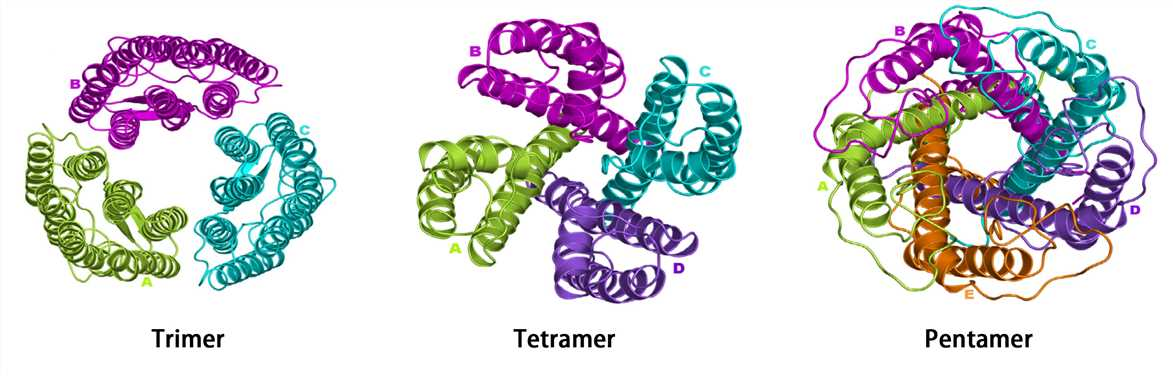
\includegraphics[scale=0.39]{images/quaternary_protein_structure.jpg}
\end{center}
\crediturl{Image}{https://www.creative-biostructure.com/levels-of-protein-structure.htm}
\begin{itemize}
	\item Composition of multiple polypeptide (amino acids) chains
	\item Only in some proteins
\end{itemize}
\end{frame}